\documentclass[12pt]{standalone}

\usepackage{tikz}

\tikzset{real edge/.style={black,solid,very thick}}
\tikzset{virtual edge/.style={black,dashed,thin}}

\begin{document}
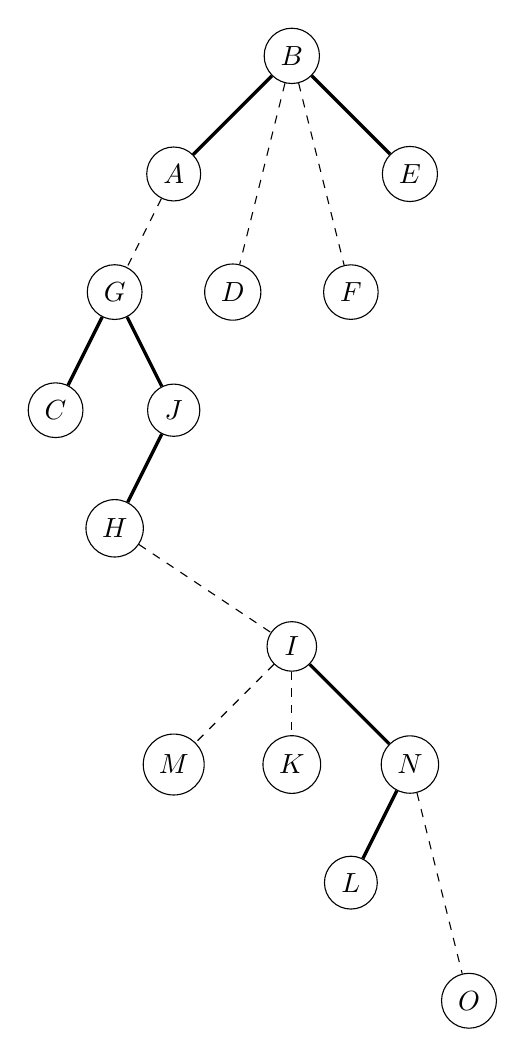
\begin{tikzpicture}[x=1.5cm,y=1.5cm]

\begin{scope}[real edge,every node/.style={black,solid,thin,circle,draw}]

\node (B) at (0,5) {$B$}
    child {node (A) {$A$}}
    child[missing]
    child {node (E) {$E$}};

\node (D) at (-0.5,3) {$D$};

\node (F) at (0.5,3) {$F$};

\node (G) at (-1.5,3) {$G$}
    child {node (C) {$C$}}
    child {node (J) {$J$}
        child {node (H) {$H$}}
        child[missing]};

\node (I) at (0,0) {$I$}
    child[missing]
    child[missing]
    child {node (N) {$N$}
        child {node (L) {$L$}}
        child[missing]};

\node (K) at (0,-1) {$K$};

\node (M) at (-1,-1) {$M$};

\node (O) at (1.5,-3) {$O$};

\end{scope}

\draw[virtual edge]
    (B) edge (D)
    (B) edge (F)
    (A) edge (G)
    (H) edge (I)
    (I) edge (K)
    (I) edge (M)
    (N) edge (O);

\end{tikzpicture}
\end{document}
